\documentclass[journal,12pt,twocolumn]{IEEEtran}
\usepackage{tikz}
\usepackage{amsmath}
\usepackage{amssymb}
\pagestyle{empty}
\usepackage{setspace}
\singlespacing
\usepackage{caption}
\captionsetup{justification=centering}
\usepackage{amsthm}
\usepackage{amssymb,amsmath}


\begin{document}
\newcommand{\myvec}[1]{\ensuremath{\begin{pmatrix}#1\end{pmatrix}}}
\newcommand{\cmyvec}[1]{\ensuremath{\begin{pmatrix*}[c]#1\end{pmatrix*}}}
\providecommand{\norm}[1]{\lVert#1\rVert}
\newcommand{\mydet}[1]{\ensuremath{\begin{vmatrix}#1\end{vmatrix}}}
\newcommand{\proj}[2]{\textbf{proj}_{\vec{#1}}\vec{#2}}
\newcommand{\abs}[1]{\left\lvert#1\right\rvert}
\newcommand{\RNum}[1]{\uppercase\expandafter{\romannumeral #1\relax}}
\newcommand{\Rnum}[1]{\lowercase\expandafter{\romannumeral #1\relax}}
\let\StandardTheFigure\thefigure
\let\vec\mathbf
\title{
Assignment - 1
}
\author{BILLAKURTHI SHAI SASI DEEP\\ SM21MTECH12006}
\maketitle
\newpage
\bigskip
\bibliographystyle{IEEEtran}
\section*{ Chapter \RNum{2} Ex-\RNum{2} Q.4-\Rnum{3}}
\vspace{0.3cm}
\noindent
\textbf{Show that the following triad of points form
\vspace{0.3cm}\\
an equilateral triangle \myvec{a\\0}, \myvec{0\\2a}, \myvec{2a\\a}, axes 
\vspace{0.3cm}\\
being inclined at an angle of 60$^{\circ}$} \\
\\
\text{Answer:}  
\vspace{0.3cm}
A triangle is said to be equilateral if length of all sides are equal.
\vspace{0.6cm} 

The given points are:
\begin{align*}
\vec{A} = \myvec{a\\0}, \vec{B} =\myvec{0\\2a},
\vec{C} =\myvec{2a\\a}
\end{align*}


The distance between points A and B,
\vspace{0.3cm}
\begin{align*}
\vec{A} - \vec{B}&=\myvec{a\\0}-\myvec{0\\2a}=\myvec{a\\-2a}\\\\
\norm{\vec{A}-\vec{B}}^2 &=({\vec{A}-\vec{B}})^\top({\vec{A}-\vec{B}})\\
&= \myvec{a \ -2a} \myvec{a\\-2a}\\\\
\norm{\vec{A}-\vec{B}}&=\sqrt{(a)^2+(-2a)^2}
\end{align*}
\begin{align}
 \norm{ \vec{A}-\vec{B}}=\sqrt{5}a   \label{Eq:1}
\end{align}
Similarly, 
\begin{align*}
\vec{B} - \vec{C}&=\myvec{0\\2a}-\myvec{2a\\a}=\myvec{-2a\\a}\\\\
\norm{\vec{B}-\vec{C}}^2&=({\vec{B}-\vec{C}})^\top({\vec{B}-\vec{C}})\\&= \myvec{a \ -2a} \myvec{a\\-2a}\\\\
\norm{\vec{B}-\vec{C}}&=\sqrt{(-2a)^2+(a)^2}
\end{align*}
\begin{align}
    \norm{ \vec{B} - \vec{C}}&=\sqrt{5}a \label{Eq:2}
\end{align}
\begin{align*}
\vec{C} - \vec{A}&=\myvec{2a\\a}-\myvec{a\\0}=\myvec{a\\a}\\\\
\norm{\vec{C}-\vec{A}}^2&=({\vec{C}-\vec{A}})^\top({\vec{C}-\vec{A}})\\&= \myvec{a \ a} \myvec{a\\a}\\\\
\norm{\vec{C}-\vec{A}}&=\sqrt{(a)^2+(a)^2}
\end{align*}
\begin{align}
\norm{ \vec{C} - \vec{A}}&=\sqrt{2}a     \label{Eq:3}
\end{align}
\begin{figure}[!ht]
   \centering
   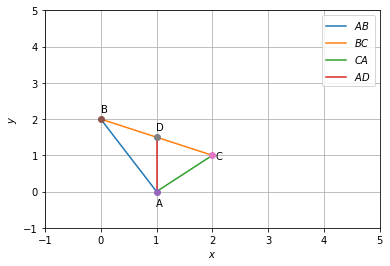
\includegraphics[width=\columnwidth]{BOP.png}
   \caption{Triangle formed for a=1}
   
\end{figure}\\
From {\eqref{Eq:1}}, {\eqref{Eq:2}}, {\eqref{Eq:3}}\\\\
$\norm{ \vec{A} - \vec{B}} = \norm{ \vec{B} - \vec{C}}  \neq \norm{ \vec{C} - \vec{A}} $ \\\\
So the given triad of points does not form an equilateral triangle.

\end{document}

\end{document}
